
\subsection{GPU acceleration reduces design runtimes}

A major performance bottleneck of \osprey designs with continuous flexibility is minimizing protein conformations and conformation fragments. Since the space of possible conformations in a design grows exponentially with the number of flexible and mutable residues, the number of conformations that must (in the worst-case) be enumerated to find the GMEC or to approximate the Boltzmann-weighted partition function grows exponentially as well. Since all enumerated conformations must be subsequently minimized to compute their energies, and minimization is a relatively expensive operation, the bulk of a design's runtime can be spent on energy minimization of conformations. Therefore, improvements to the speed of energy minimization (an operation that is called an exponential number of times) can have a dramatic impact on \osprey runtimes.

Much work has been done in the past to optimize \osprey for execution on CPUs, particularly highly multi-core CPUs and even networked clusters of CPU-powered servers~\cite{minBounds_DACS,cloud_OSPREY}. However, modern GPU hardware enables high-performance computation at a fraction of the cost of large CPU clusters, mainly due to the huge video game industry that propels innovation in hardware design and drives down costs. \osprey3 includes GPU programs (called {\it kernels}) built using the CUDA framework that implements the forcefield calculations and local minimization algorithms used in protein redesign. We present performance results of these GPU kernels on various hardware platforms in Figure~\ref{fig:gpu}. Overall, on desktop-class machines, GPU hardware improves minimizations speeds over multi-core CPUs by roughly 12-fold for sufficiently large molecules. On server-class machines, a single GPU is merely about 2.6-fold faster than dual CPUs. These large machines can house more GPUs than CPUs though, so a fully-provisioned server with 4 or even 8 GPUs would likely greatly outperform 2 or even 4 CPUs. Laptop-class GPUs, however, do not appear to be powerful enough to offer any advantages over traditional CPU computing in \osprey3.

Modern GPU architectures offer thousands of parallel hardware units for calculations, compared to the tens of parallel hardware units in modern CPU architectures. The performance results of the current incarnation of \osprey's GPU kernels indicate that current minimization speeds on GPUs have only begun to scratch the surface of what is possible, particularly for molecules with a small number of atom pairs. It is incredibly likely that future versions of these GPU kernels will offer significantly higher performance on the same hardware -- perhaps allowing minimization speeds many times faster than today's GPU kernels.

\begin{figure}\label{fig:gpu}
\center
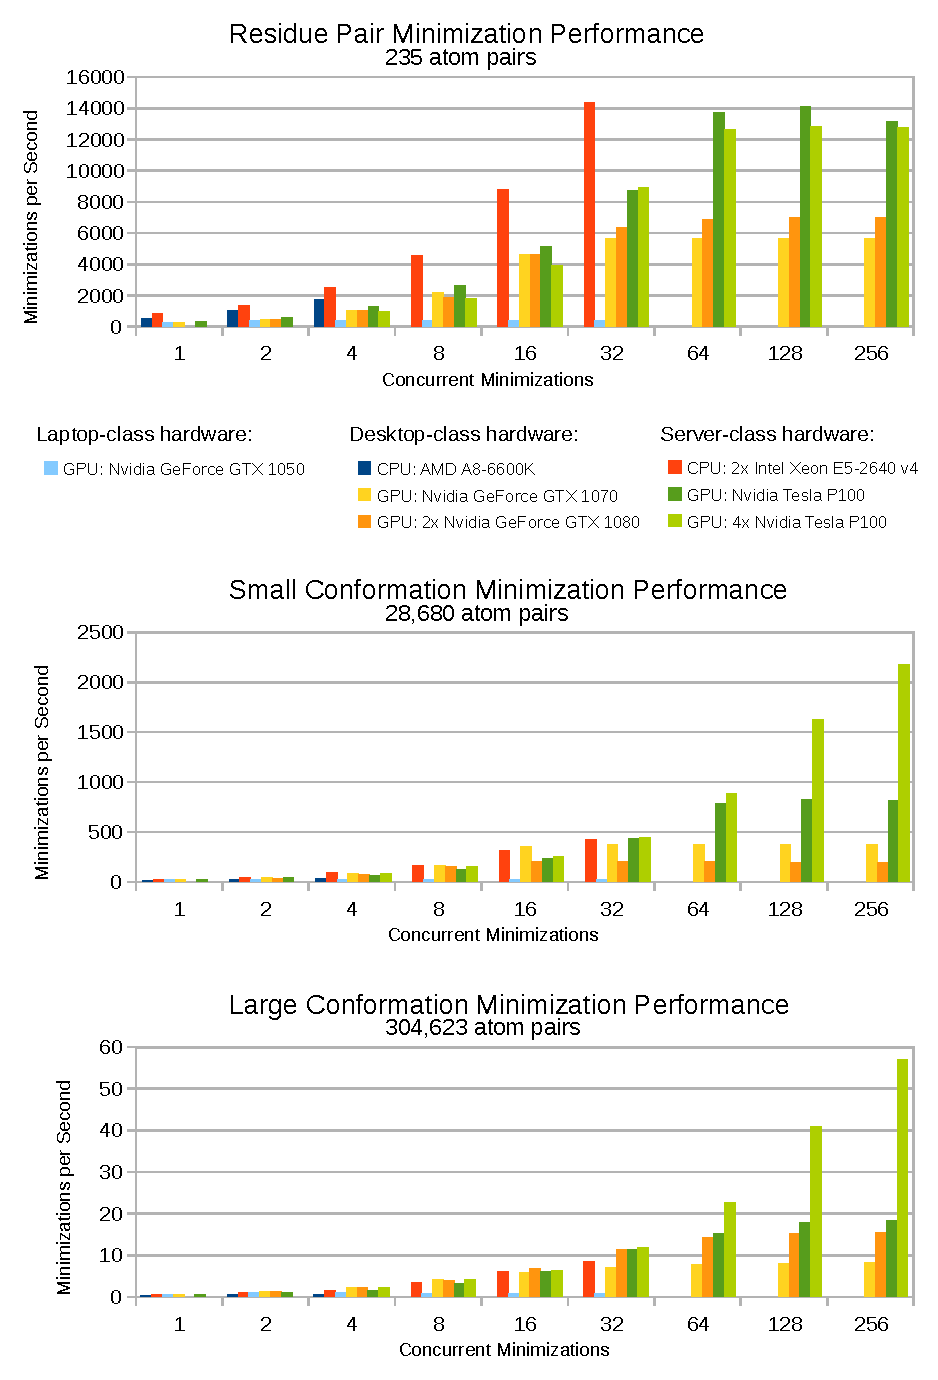
\includegraphics[width=4in]{figures/gpu.pdf}
\caption{Benchmarks for protein conformation minimization in \osprey3 for various hardware platforms and for molecules of varying size. From smallest to largest: {\bf (top)} a single residue pair used in energy matrix computations, {\bf (middle)} a full protein conformation with a single flexible residue, {\bf (bottom)} a full protein conformation with 20 flexible residues. For CPU hardware, concurrent minimizations correspond to CPU threads. For GPU hardware, concurrent minimizations correspond to {\it streams} defined by the CUDA framework. Faster minimization speeds correspond with faster \osprey runtimes.}
\end{figure}
